\documentclass[12pt,fleqn]{article}
\setlength{\parindent}{0pt}
\usepackage{graphicx}
\usepackage{listings}
\usepackage[latin5]{inputenc}
\setlength{\parskip}{8pt}
\setlength{\parsep}{0pt}
\setlength{\headsep}{0pt}
\setlength{\topskip}{0pt}
\setlength{\topmargin}{0pt}
\setlength{\topsep}{0pt}
\setlength{\partopsep}{0pt}
\setlength{\mathindent}{0cm}

\begin{document}
MIT OCW Cok Degiskenli Calculus - Ders 4

Duzlemin formulune donelim. 

\[ ax + by + cz = d \]

Bu formul $x,y,z$ noktalarinin bir duzlem uzerinde olma sartini tarif
ediyor. 

Su problemlere bakalim. Diyelim ki 

1) Orijinden gecen ve normal vektoru $\vec{N} = <1,5,10>$ olan bir duzlem
yaratmek istiyoruz. Yani alttaki gibi bir sekil:

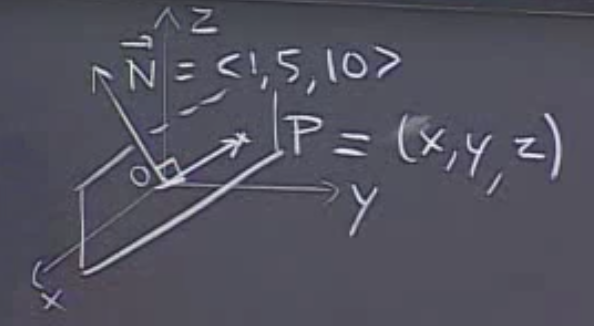
\includegraphics[height=4cm]{4_1.png}

Herhangi bir nokta $P = (x,y,z)$  ne zaman bu duzlem uzerindedir? Eger
orijinden $P$'ye giden vektor, duzlem normali ile doksan derece aci
olusturuyorsa. Yani $\vec{OP} \cdot \vec{N} = 0$ oldugu zaman $P$ noktasi
duzlem uzerindedir. Bu carpimi normal icin verdigimiz ornek sayilar icin
yaparsak, sonuc $x+5y+10 = 0$ olacaktir. 

2) Simdi duzlem $P_0 = (2,1,-1)$ noktasindan gecsin (orijinden degil), ve
normal yine ayni olsun, $\vec{N} = <1,5,10>$. Bu durumu zihnimizde
canlandirmak icin orjinden gecen degil, yeni bir duzlemi hayal etmemiz
lazim, ve $P$ noktasi bu yeni duzlem uzerinde olacak. 

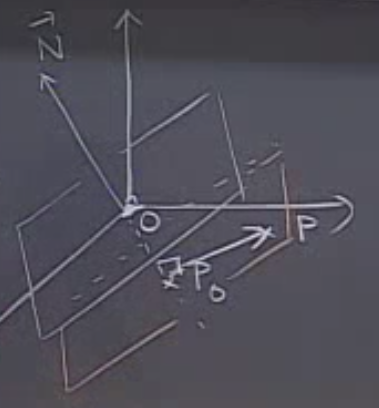
\includegraphics[height=4cm]{4_2.png}

$P$ ne zaman duzlem uzerinde? Eger 

\[ \vec{P_0P} \cdot \vec{N} = 0 \]

ise. O zaman 

\[ <x-2, y-1, z+1> \cdot <1,5,10> = 0 \]

\[ x+5y + 10z = -3 \]

1. problemdeki sonuctakiyle aradaki tek fark esitligin sagindaki -3
degeri. Bir benzerlik ise her iki durumda da $x,y,z$ katsayilarinin normal
vektorun degerlerine tekabul ediyor olmasi. Bu duzlemler hakkinda onemli
bir puf noktasi, eger orjinden geciyorlarsa esitligin sag tarafi sifir,
baska bir yerden geciyorlarsa, baska bir deger. Peki bu -3 degerini daha
hizli bir sekilde bulamaz miydik? Bulabilirdik. Cunku esitligin sol
tarafinin katsayilarini hizli bir sekilde bulabiliyoruz, orasi
tamam. Ayrica duzlemdeki bir noktanin kordinatlarini da biliyoruz, bu nokta
duzlemin icinden gecmesini sart kostugumuz $P_0$ noktasi. O zaman bu
kordinati $x,y,z$ terimlerini iceren formule koyarsak, esitligin sag
tarafini hemen hesaplariz. 

\[ x+5y + 10z = 1(2) + 5(1) + 10(-1) = 2 + 5 -10 = -3\]




\end{document}
